\documentclass[../main/main.tex]{subfiles}


\begin{document}

\section{February 12th, 2020}
\subsection{Example Mass/Spring/Damper System}
We have a mass $m>0$ attached to a spring with spring coefficient $k>0$ and a dampener with coefficient $b\ge 0$. If we assume no coefficient of friction, we get \[
	-k-x-b\dot{x} = m\ddot{x}
.\] Which can be rearranged to: \[
m\ddot{x} + b\dot{x}+kx=0
.\] Which is a 2nd-order linear homogeneous ODE with constant coefficients, which we can use the table from earlier to solve. If we include an external force acting on the mass, we would have:
\begin{equation} \label{mass}
m\ddot{x}+b\dot{x}+kx=F(t) 
\end{equation}
Which would make it non homogeneous. There is an analog circuit equivalent called the LCR circuit, which would have an equation: \[
L\ddot{Q}+R\dot{Q}+\frac{1}{C}Q=\Delta V
.\] Which is of the same form as Equation \ref{mass}.

Let us consider the case without a driving force $F(t)$:  \[
	\ddot{x}+\frac{b}{m}\dot{x}+\frac{k}{m}x=0
	.\]First, we will denote $\omega=\sqrt{\frac{k}{m}} $ which represents the \vocab{angular frequency}\index{angular frequency} of the system, with units rad per sec, and $\gamma=\frac{b}{2\sqrt{m k }}$ be a \vocab{dampening ratio}\index{dampening ratio} (which represents how much dampening is in the system), making the equation: \[ 
	\ddot{x}+2\gamma\omega\dot{x}+\omega^2x=0
.\] Note that discriminant of this equation is: \[
D= \frac{b^2}{m^2}  -4 \frac{k}{m} = \frac{4k}{m}\left( \frac{b^2}{4\sqrt{m k} }-1 \right) = 4\omega^2(\gamma^2-1) 
.\] Now depending on what $\gamma$ and  $\omega$ are, we can analyze the behaviour of the system.
\subsection{No Dampening ($\gamma=0$)} 
In this case, we would have: \[
	\ddot{x}+\omega^2x=0
.\] The discriminant is thus: \[
D=0^2-4(1)(\omega^2)=-4\omega^2<0
.\] Using the table, we have: \[
\alpha=-\frac{0}{2(1)}=0, \quad\beta = \frac{\sqrt{-(-4\omega^2)}}{2(1)} = \omega
.\] Thus the solution will just be: \[
x(t) = c_1\cos(\omega t)+c_2\sin(\omega t)
.\] If we want to find the constants, note that $x(0)=x_0=c_1$. Meanwhile, differentiating the equation, we have: \[
v(t) = -c_1\omega\sin(\omega t)+\omega c_2(\omega t) 
.\] \[
v(0)=v_0=\omega c_2
.\] Thus the complete solution is: \[
x(t) = x_0 \cos(\omega t) + \frac{v_0}{\omega}\sin(\omega t)
.\] 
\begin{figure}[h!]
	\centering
	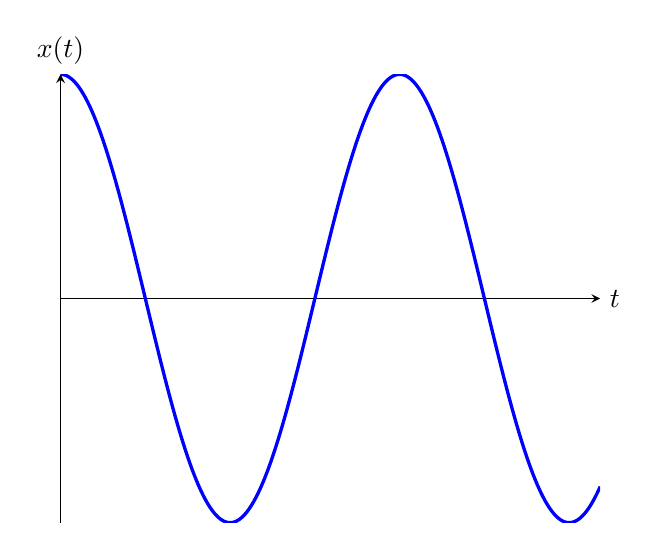
\begin{tikzpicture}
    \begin{axis}[domain=0:5,samples=501,axis lines=center,
    xtick=\empty,ytick=\empty,
    xlabel={$t$},xlabel style={anchor=west},
    ylabel={$x(t)$},ylabel style={anchor=south}]
	\addplot[color=blue,no marks,very thick,smooth] {cos(2*deg(x)};
    \end{axis}
\end{tikzpicture}
	\caption{ Example of Underdamped Motion}
	\label{fig:}
\end{figure}
This is just a sin curve with amplitude: $A=\sqrt{x_0^2+\left( \frac{v_0}{\omega} \right) ^2} $ and period: $T=\frac{2\pi}{\omega}$.
\begin{remark}
	Note that the period does not depend on $x_0$ or $v_0$, i.e. it doesn't depend on how it starts. This is different from SHM.
\end{remark}
\subsection{Under Damping ($0<\gamma<1$)}
Returning to our equation, we have: \[
	\ddot{x} + 2\gamma\omega \dot{x} + \omega^2x = 0
.\] Thus the determinant is: \[
D=(2\gamma\omega)^2-4(1)(\omega^2)=4w^2(\gamma^2-1)
.\] If $0<\gamma<1$, we have $D<0$, giving us:  \[
\alpha = \frac{-(2\gamma\omega)}{2(1)}=-\gamma\omega,\quad \beta=\frac{\sqrt{-D} }{2(1)}=\omega\sqrt{1-\gamma^2} 
.\] Plugging this into the equation, we get: \[
x(t) = c_1 e^{-\gamma\omega t}\cos(\omega t\sqrt{1-\gamma^2} ) +c_2 e^{-\gamma\omega t}\sin(\omega t\sqrt{1-\gamma^2} )
.\]
\begin{figure}[h!]
	\centering
	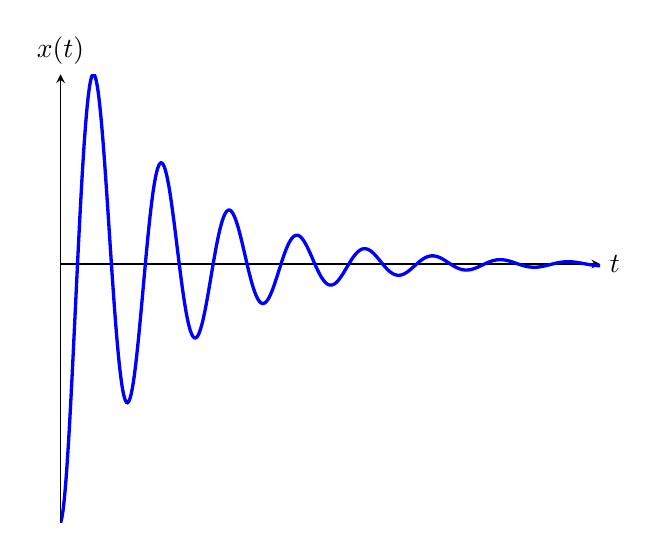
\begin{tikzpicture}
    \begin{axis}[domain=0:5,samples=501,axis lines=center,
    xtick=\empty,ytick=\empty,
    xlabel={$t$},xlabel style={anchor=west},
    ylabel={$x(t)$},ylabel style={anchor=south}]
    \addplot[color=blue,no marks,very thick,smooth] {(-exp(-x)*cos(10*deg(x)))};
    \end{axis}
\end{tikzpicture}
	\caption{ Example of Underdamped Motion}
	\label{fig:}
\end{figure}
\begin{remark}
	Note that there will be infinite oscillations where the amplitude is decreasing to 0.
\end{remark}
\subsection{Critical Damping ($\gamma=1$)} \index{critical dampening}
Notice in the case of $\gamma=1$, we have $D=0$, thus the solution is:  \[
	x(t) = c_1 e^{-\gamma\omega t}+c_2te^{-\gamma\omega t}
.\] 
\begin{figure}[htpb]
	\centering
	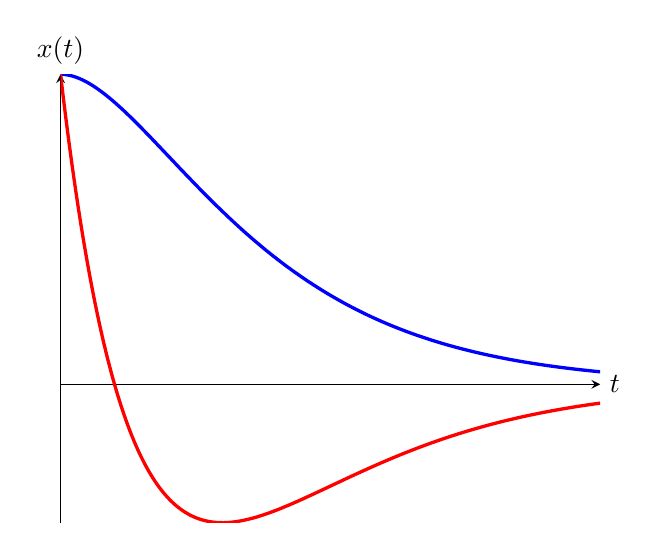
\begin{tikzpicture}
    \begin{axis}[domain=0:5,samples=501,axis lines=center,
    xtick=\empty,ytick=\empty,
    xlabel={$t$},xlabel style={anchor=west},
    ylabel={$x(t)$},ylabel style={anchor=south}]
	\addplot[color=blue,no marks,very thick,smooth] {((0.5+0.5*x)*exp(-x))};
	\addplot[color=red,no marks,very thick,smooth] {((0.5-x)*exp(-x))};
    \end{axis}
\end{tikzpicture}
	\caption{ Example of Critical Damped / Over Damped Motion}
	\label{fig:}
\end{figure}
\begin{remark}
	Note that in this case, there are no oscillations. There will never be two dips. This is because we have: \[
		x(t) = c_1e^{-\gamma\omega t}+c_2te^{-\gamma\omega t} = (c_1+c_2 t)e^{-\gamma\omega t}
	.\]  Thus by looking at the sign of $c_1$ and $c_2$, it will either never cross the $x$ axis (if same sign) or only cross it once (if signs are different). This can be shown by looking at the roots of the equation above.
\end{remark}

\subsection{Over Damping ($\gamma>1$)}\index{over damping}
This yields $D>0$, thus: \[
	x(t) = c_1e^{-\gamma\omega t} \cosh(\gamma t\sqrt{\gamma-1} ) + c_2 e^{-\gamma\omega t}\sinh(\omega t\sqrt{\gamma^2-1} )
.\] 
\begin{remark}
	This is the case where we are taking away the energy a lot, which is useful in many cases. This will make it go to 0 a lot faster than critical damping. Thus for car suspension, we would rather it be critically damped than over damped.
\end{remark}

\begin{remark}
	In circuits, this is analogous to using resistors to take away heat from the circuit.
\end{remark}

\subsection{Laplace Transforms}
Laplace transforms are a special case of integral transforms. One way to think of an integral transform is that it's a function where the input is a function of $t$ and output a function of $s$.
\begin{definition}
	More specifically, a \vocab{integral transform}\index{integral transform} is of form: \[
		\int_{\alpha(s)}^{\beta(s)} f(t) K(s,t)~dt
	.\] Where $K(s,t)$ is the \vocab{kernel}\index{kernel} of the transform, and $\alpha(s)$ and $\beta(s)$ are the upper and lower limit.
\end{definition}
\begin{example}
	Consider the case where $\alpha(s)=s,\ \beta(s)=s^2,\ K(s,t) = st$, and an input $f(t) = t^3$. Then the output would be:  \[
		\int_{s}^{s^2}t ^{3}(st)~dt = \frac{st^{5}}{5}\bigg\rvert_{t=s}^{t=s^2}=\frac{1}{5}\left( s^{11}-s^{6} \right) =F(s)
	.\] 
\end{example}
\begin{definition}
	Typically, we represent this integral transform as $T\{f(t)\}=F(s)$.
\end{definition}
\begin{definition}
	The \vocab{Laplace Transform}\index{Laplace transform} is a special case where: \[
		\alpha(s)=0\quad\beta(s)=\infty\quad K(s,t) = e^{-st}
	,\] in other words: \[
	\mathcal{L}\{f(t)\} = \int_0^\infty f(t) e^{-st}~dt = F(s)
	.\]  
\end{definition}
\begin{remark}
	Note that $st$ must be unitless, and if  $t$ represents time, then $s$ represents frequency, thus making the Laplace transform a transformation from time space into frequency space.
\end{remark}
\begin{example}
	We have\[
	\mathcal{L}\{1\} = \int^\infty_0 e^{-st}~dt = \frac{e^{-st}}{-s}\bigg\rvert_0^\infty=\frac{1}{s}
	.\] Note that $s>0$
\end{example}
In order to go from $s$-space back to $t$-space, we take the inverse Laplace transform. This will be unique as long as we don't consider null functions.
\begin{definition}
	A \vocab{null function}\index{null function} is a function that is zero except for finitely many points.
\end{definition}
\begin{example}
	An example of a null function is: \[
		N(t) = \begin{cases}
			1,\quad t=0\\
			2,\quad t=1\\
			0,\quad \text{otherwise}
		\end{cases}
	.\] 
\end{example}
These null functions do not appear often for our situation, so we can have a Laplace transform table: 

\begin{table}[htpb]
	\centering
	\caption{Laplace Transform Table}
	\begin{tabular}{c|c|c}
	 1& $\frac{1}{s}$ & $s>0$\\
	 \hline
	 $e^{at}$& $\frac{1}{s-a}$ & $s>a$\\
	 \hline
	 $\sin(\omega t)$& $\frac{\omega}{s^2+\omega^2}$ & $s>0$\\
	 \hline
	 $\cos(\omega t)$& $\frac{s}{s^2+\omega^2}$ & $s>0$\\
	 \hline
					 &$\vdots$&
	\end{tabular}
\end{table}
\begin{remark}
	Using the table, one example is: $\mathcal{L}^{-1}\left\{ \frac{s}{s^2+\omega^2}\right\}$
\end{remark}

\end{document}

